\sloppy
\documentclass[11pt, openany, a4paper]{book}

%\usepackage[utf8]{inputenc}
%\usepackage[russian]{babel}


\usepackage{polyglossia}
\setmainlanguage{russian}
\setotherlanguage{english}
\setkeys{russian}{babelshorthands=true}

\newfontfamily{\cyrillicfont}{Times New Roman} 
\newfontfamily{\cyrillicfontrm}{Times New Roman}
\newfontfamily{\cyrillicfonttt}{Courier New}
\newfontfamily{\cyrillicfontsf}{Arial}

\addto\captionsrussian{%
  \renewcommand{\figurename}{Рис.}%
  \renewcommand{\tablename}{Табл.}%
}


\usepackage{amsmath}
\usepackage{amssymb}
\usepackage{amsthm}
\usepackage[final]{graphicx}
\usepackage{fancyhdr}
\usepackage{epigraph}
\usepackage{floatflt}
\usepackage{mathtext}
\setlength{\textwidth}{170mm}\setlength{\textheight}{240mm}
\topmargin=-10mm
\oddsidemargin=-3mm
\evensidemargin=-3mm
\renewcommand{\chaptermark}[1]{\markboth{#1}{}}
\renewcommand{\sectionmark}[1]{\markright{\thesection\ #1}}
\fancyhf{}  % убираем текущие установки для колонтитулов
\fancyhead[LE,RO]{\thepage}
\fancyhead[LO]{\itshape\rightmark}
\fancyhead[RE]{\itshape\leftmark}
\renewcommand{\headrulewidth}{0.5pt}
\renewcommand{\footrulewidth}{0pt}
\addtolength{\headheight}{5pt}
\newfont\TTT{larm1200 scaled 2000}
\newfont\AAA{larm1095 scaled 1500}
\def\AmSTeX{{\the\textfont2 A}\kern-.1667em\lower.5ex\hbox
{\the\textfont2 M}\kern-.125em{\the\textfont2 S}-\TeX}
\newcounter{Fig}\setcounter{Fig}{0}
\newcommand{\Ris}[1]{рис.~\ref{fig:#1}}
\newcommand{\Caption}[2]{\stepcounter{Fig}\caption{\label{fig:#1}#2}}
\newcommand{\Paragraph}[1]{\par\vspace{2mm}\noindent{\bf{}#1}\vspace{2mm}\par{}}
\newcommand{\Sec}[1]{см.\ раздел\ref{sec:#1}}
\newcommand{\Term}[2]{\item[#1]\label{abb:#2} --- }
\newcommand{\SeeTerm}[1]{см.\ статьи из глоссария на стр.\ \pageref{abb:#1}}
\graphicspath {{./img/}}
\includeonly  
{
	zadachi,
	File_2,
	oblozjka,
}
\makeindex

%%чего не хватило российской науке во время пандемии Подробнее на РБК:
%%https://www.rbc.ru/opinions/society/23/05/2020/5ec79db29a794732c603b1ce

\begin{document}

\tableofcontents
    \newpage
\section{Черновик задач}

\subsection{Оператор присваивания}

\begin{enumerate}
  \item Дано $A, B$,
    \begin{enumerate}
      \item Обменять значения переменных
      \item Обменять значения переменных, не используя дополнительную переменную.
    \end{enumerate}

  \item Найти расстояние между двумя точками, заданными координатами в двумерном пространстве.

  \item Вычислить площадь треугольника, если даны координаты его вершин.

  \item Дано целое число $A$. Вычислить $A^15$ за минимальное количество операций умножения. (Деление не использовать)
\end{enumerate}

\subsection{Условный оператор}

\begin{enumerate}
  \item Даны два числа $A$ и $B$. Найти минимумальное и максимумальное значениие.

  \item Даны три числа $A$, $B$ и $C$. Найти минимумальное и максимумальное значениие.

  \item Найти минимум из 4 заданных чисел за минимальное количество операций сравнения.

  \item Найти максимум из 4 заданных чисел за минимальное количество операций сравнения.
\end{enumerate}

\subsection{Операции целочисленного деления}

\begin{enumerate}
  \item Дано целое число. Определить четное оно или нет.

  \item Дано целое двухзначное целое число, найти сумму цифр этого числа.

  \item Дано целое трёхзначное целое число, найти сумму цифр этого числа.

  \item Дано целое число байт, разложить его на Гб, Мб, Кб, байты.

  \item Даны координаты двух клеток на бесконечной шашматной доске. Координаты - пара целых чисел. Определить одного цвета клетки или разного. (Цвет клеток определять не требуется)
\end{enumerate}

\subsection{Операторы цикла}

\begin{enumerate}
  \item Вычислить $N! = 1*2*3*...*N$ по очереди всеми типами циклов. (for, while, repeat until)

  \item Вычислить $X^N$, где N - целое не отрицательное.

  \item Дана последовательность целых чисел. Определить на какую максимальную степень числа 3 делится хотя бы одно из чисел.

  \item Вывести все делители числа.

  \item Определить, является ли введенное число простым.

  \item Вывести все простые числа из интервала от 1 до 100.

  \item Вывести первые $M$ простых чисел. $M$ задается с клавиатуры.

  \item Найти НОД(А, В), используя формулу НОД(А, В) = НОД(В, А mod В)
  
  \item Наименьшее общее кратное двух целых чисел находится по формуле $HOK(A,B)=\frac{A*B}{HOD(A,B)}$, где $HOD$ --- наибольший общий делитель. Написать программу, которая находит наименьшее общее кратное заданных чисел.

  \item Определить является ли введенное число числом Фибоначчи.
\end{enumerate}

\subsection{Массивы}

Заполнить массив из 10 элементов случайными целыми числами из отрезка [M, N].

Найти:
\begin{enumerate}
  \item Найти минимальное и максимальное значение элемента массива.
  \item Найти сумму чётных значений элементов массива.
  \item Найти количество отрицательных элементов массива и их среднее арифметическое.
  \item Вывести номера элементов массива, которые являются локальными минимумами. Для локального минимума выполнено условие $x[i-1] > x[i] < x[i+1]$.
  \item Найти максимум среди локальных минимумов.
\end{enumerate}

\subsection{Строки как массивы}

\begin{enumerate}
  \item Дана строка. Определить количество цифр в ней.
  \item Дана строка. Заменить в ней все вхождения символа А на В.
  \item Определить является ли введенная строка целым числом.
  \item Определить является ли введенная строка вещественным числом.
  \item Посчитать количество вхождений каждого символа в строке.
\end{enumerate}

\subsection{Строки}

\begin{enumerate}
  \item Дан символ C и строки S, S0. Перед каждым вхождением символа C в строку S вставить строку S0.
  \item Даны строки S и S0. Проверить, содержится ли строка S0 в строке S.
  \item Даны строки S и S0. Удалить из строки S все подстроки, совпадающие с S0.
  \item Даны строки S, S1 и S2. Заменить в строке S все вхождения строки S1 на строку S2.
  \item Вычислить количество слов в заданной строке. Слова разделены пробелами.
  \item Определить длину самого длинного слова в строке. Вывести это слово и его длину.
  \item Найти в строке слово, являющееся палиндромом. (Например ТОПОТ)
  \item Дана строка, построить строку, содержащую только слова с нечетными номерами.
  \item Определить какое количество раз в заданной строке встречается первое слово.
  \item Дана строка, содержащая арифметическое выражение. Написать программу “Калькулятор”. Калькулятор должен уметь:
     \begin{enumerate}
       \item вычислять значение выражения, содержащего два числа и знак операции между ними (Например “4+2”);
       \item вычислять значение произвольного выражения без скобок, с учетом порядка действий;
       \item вычислять значение выражения со скобками, с учетом порядка действий;
       \item вычислять значение выражения, содержащего скобки и основные тригонометрические функции.
     \end{enumerate}
  \item Дано $k$, $m$, $X$ - целые числа. Найти значение Y, если известно, что $X_k=Y_m$. (Перевести число $X$  из $k$-теричной системы исчисления в $m$-теричную). $2<=k,m<=10$
\end{enumerate}


\subsection{Подготовка к ЕГЭ}

{\bf Задание №1}

Дан список точек плоскости с целочисленными координатами. Необходимо определить:
\begin{enumerate}
  \item номер координатной четверти K, в которой находится больше всего точек;
  \item точку A в этой четверти, наименее удалённую от осей координат;
  \item расстояние R от этой точки до ближайшей оси.
\end{enumerate}
  
Если в нескольких четвертях расположено одинаковое количество точек, следует выбрать ту четверть, в которой величина R меньше. При равенстве и количества точек, и величины R необходимо выбрать четверть с меньшим номером K. 
Если в выбранной четверти несколько точек находятся на одинаковом минимальном расстоянии от осей координат, нужно выбрать
первую по списку. Точки, хотя бы одна из координат которых равна нулю, считаются не принадлежащими ни одной четверти и не рассматриваются. Напишите эффективную, в том числе по памяти, программу, которая будет решать эту задачу.
В первой строке вводится одно целое положительное число – количество точек N. Каждая из следующих N строк содержит координаты очередной точки – два целых числа (первое – координата x, второе – координата y).

Пример входных данных:
\begin{verbatim}
7
-3 4
1 2
1 1
0 4
-2 -3
-6 8
-12 1
\end{verbatim}

Пример выходных данных для приведённого выше примера входных данных:
\begin{verbatim}
K = 2
A = (-12, 1)
R = 1
\end{verbatim}


{\bf Задание №2}

На прямоугольном поле для игры в морской бой размером M×N расположено несколько прямоугольных кораблей. Корабли не соприкасаются друг с другом. Ваша задача — определить всевозможные типы кораблей на поле и число кораблей каждого типа. 
Два корабля относятся к одному типу, если их размеры совпадают (корабли, которые могут быть получены друг из друга поворотом, также относятся к одному типу).
Входные данные
Первая строка входных данных содержит два положительных числа M и N, не превосходящих 1000, задающие размеры поля. Далее идет M строк, каждая из которых состоит из N символов. 
Символ `1' означает, что соответствующая клетка поля занята кораблем, символ `0' — что свободна. Пробелов в строке нет.
Выходные данные
Программа должна для каждого обнаруженного типа корабля вывести одну строку, содержащую три числа. Первые два числа задают размеры корабля (первое число должно быть не меньше второго), 
третье число задает количество кораблей данного типа на поле. Строки в выводе должны быть отсортированы по первому числу, затем по второму числу.

Пример входных данных
\begin{verbatim}
    6 10
    0111000011
    0000011011
    0100011000
    0101011011
    0100000000
    0001111011
\end{verbatim}

Пример выходных данных
\begin{verbatim}
    1 1 1
    2 1 2
    2 2 2
    3 1 2
    3 2 1
    4 1 1
\end{verbatim}



{\bf Задание №3}

Решил как-то Иванушка-дурачок навестить Змея Горыныча. Пришел он к замку, а перед воротами минное поле раскинулось. Причем поле не простое, а волшебное – мины расположены в узлах регулярной решетки. 
Однако, была у Иванушки лягушка-сапер, работающая по следующему алгоритму. Лягушка прыгает с мины на мину, разряжая ту, на которой сидит. Если она видит, что перед ней нет мины, или мина перед ней разряжена, 
она поворачивается на 90 градусов вправо. Если вокруг лягушки не остается заряженных мин, то она останавливается. Перед тем как запускать свою лягушку, решил Иванушка определить где она остановится. 
Для этого он ввел систему координат, причем ось x оказалась направлена вправо, а ось y – вверх. Потом он обнаружил, что мины оказались расположены в точках с координатами (i, j), причем $1 < i < N$; $1 \le i \le N$, $1 < j < M$; $1 \le j \le M$, 
а лягушка изначально находится в точке (1,1) и смотрит по оси y. Требуется определить координаты точки, в которой остановится лягушка.
Входные данные
Программа получает на вход два натуральных числа N и M, не превосходящие $10^6$.
Выходные данные
Программа должна вывести два натуральных числа – координаты точки, где остановится лягушка.
Пример входных данных
\begin{verbatim}
    3 4
\end{verbatim}

Пример выходных данных
\begin{verbatim}
    2 3
\end{verbatim}



Троллейбусы одного маршрута проходят через остановку каждые k ($1 \le k<500$) минут. Известны времена прихода пассажиров на эту остановку. Если пассажир приходит на остановку в момент прихода троллейбуса, то он успевает уехать на нем.
Напишите программу, которая бы определяла, во сколько должен пройти первый троллейбус (это время от 0 до k-1), чтобы:
1) Суммарное время ожидания троллейбуса для всех пассажиров было минимально.
2) Максимальное из времен ожидания троллейбуса было минимально.
Формат входных данных
Во входном потоке записано сначала число k, затем – число N ($0 \le N < 100000$). Затем идет N чисел, задающих времена прихода пассажиров на остановку. Каждое из этих чисел – целое от 0 до 100000.
Формат выходных данных
Программа должна вывести два числа, являющиеся ответами на первый и второй вопросы задачи соответственно. Если решений несколько, выведите любое из них.
Пример входных данных
\begin{verbatim}
    100 5
     0 210 99 551 99
\end{verbatim}

Пример выходных данных
\begin{verbatim}
    10
     51
\end{verbatim}


\section{Работа в среде  Pascal}

В этом практикуме стоит обратить внимание на следующие базовые понятия - компиляция и отладка программы; интегрированная диалоговая среда.

Для первоначального знакомства со средой программирования Pascal нам необходимо научиться:
\begin{itemize}
	\item вызывать интегрированную диалоговую среду Pascal и уметь выходить из нее;
	\item вводить текст программы, редактировать его и сохранять в файле с заданным именем;
	\item запускать компиляцию набранной программы;
	\item запускать программу на выполнение;
	\item включать/выключать окно вывода результатов работы программы;
	\item запускать программу в режиме отладчика;
	\item сохранять результаты счета.
\end{itemize}

Научиться выполнять указанные действия в среде Pascal можно на примере следующих заданий.

\subsection{Решение задач на языке Pascal}

Основными понятиями данного практикума являются: переменная и константа; тип и структура данных; оператор; программа (процедура, функция).

Прежде чем перейти к решению задач на языке Pascal, ответьте на следующие вопросы.

{\bf Контрольные вопросы:}
\begin{enumerate}
\item Какие символы языка Pascal Вы знаете?
\item Что такое "служебное слово"? 
\item Для чего предназначено "имя--идентификатор" и как оно записывается?
\item Что относится к элементам данных? 
\item Каковы составные части программы, написанной на языке Pascal?
\item Для чего предназначен раздел описаний?
\item В каком виде оформляются комментарии?
\item Какие стандартные типы данных Вам известны?
\item В чем отличие данных действительного и целого типов?
\item Какие значения могут принимать данные логического типа?
\item Какие логические операции Вы знаете?
\item Что такое операции отношения?
\item Что понимается под символьными данными?
\item Как описываются в программе константы, обозначаемые именами?
\item Как описываются переменные, используемые в программе?
\item Что понимается под стандартными функциями?
\item Какие стандартные функции для работы с арифметическими и символьными данными Вы знаете?
\item Каковы правила записи арифметических выражений и каков порядок их выполнения?
\item В чем отличие логического выражения от арифметического?
\item Каков порядок выполнения логического выражения?
\item Для чего предназначен оператор присваивания?
\item Чему равно значение Y после выполнения следующих операторов: $Y:=1; A:=5 - Y; Y:=Y + 2*A;$
\item Перечислите константы, используемые в следующих опера­торах: $A:=3; B15:=7; Y2:=2*A - 4*B_1;$
\item Перечислите переменные в операторе присваивания
$SUMMA:= SQR(X) + 3*A;$
\item Для чего предназначен оператор ввода?
\item Может ли быть константа параметром оператора ввода?
\item Для чего предназначен оператор вывода?
\item Каков смысл следующих предложений языка Pascal:\\
(*Вывод результатов*) \\Write('Вывод результатов');
\item Что такое составной оператор?
\item Какие основные конструкции языка Pascal Вы знаете?
\item Для чего предназначен оператор выбора?
\item Какие формы записи условного оператора Вы знаете?
\item Может ли условный оператор содержать в себе другие условные операторы?
\item Может ли условный оператор содержать оператор пере­хода?
\item Каково назначение оператора цикла?
\item Укажите основные операторы цикла в языке Pascal.
\item В чем разница всех трех операторов цикла в языке Pascal?
\item Будет ли выполняться циклическая часть программы, если логическое выражение в заголовке оператора цикла While является ложным с самого начала?
\item Можно ли изменить программным путем параметр цикла в теле цикла оператора For?
\item Чему может быть равен шаг изменения параметра цикла в операторе For?
\item Будет ли выполняться тело цикла, если логическое выра­жение в заголовке оператора Repeat истинно с самого начала?
\item Какими символами разделяются числа друг от друга при вводе оператором Read?
\item В чем особенность ввода символьных данных?
\item Что представляют собой форматы вывода?
\item В каком виде предстанут данные, если в операторе вывода форматы не указаны?
\item Для чего предназначен оператор ввода без параметров ReadLn?
\item Как организовать вывод в строке пустых позиций между данными?
\item Как организовать вывод текстовых сообщений?
\item Что такое подпрограмма?
\item Как организовать вывод текстовых сообщений?
\item В чем особенности оформления подпрограммы в виде про­цедуры и функции?
\item Что такое формальные и фактические параметры и какова связь между ними?
\item Как организовать вывод текстовых сообщений?
\item Можно ли написать процедуру без параметров?
\item Как вы понимаете локальные и глобальные переменные?
\item В чем отличия текстового и графического режимов языка Pascal?
\item Что определяют параметры в операторе инициализации гра­фического режима?
\item Что такое Crt, GraphABC и OglGraph?
\item Можно ли осуществить управление движением объекта на экране монитора в языке Pascal без использования Crt?
\item Можно ли одновременно работать в графическом и текстовом режимах языка Pascal?
\item Какими способами можно осуществить движение объекта по экрану монитора?
\item В чем особенность окончания текстов программы и подпрограммы в языке Pascal?
\end{enumerate}

Для закрепления теоретического материала по языку Pascal предлагается самостоятельно решить одну из представленных ниже задач.

\section{Задачи по программированию}

{\bf Задание №1}

Перед тем, как мы приступим непосредственно к решению задач на компьютере и познакомимся с теми инструментальными средствами, которые будут нам в дальнейшем необходимы, попро­буем научиться разрабатывать алгоритмы решения задач.

Пример поэтапного решения задачи на компьютере описан в учебном пособии для задачи о заряженных частях капли дождя. Здесь же мы приведем {\bf типовую схему решения задачи на компьютере:}
\vspace{5mm}

\begin{tabular}{ | l | l | l | }
\hline
1 & {\bf постановка задачи} & a) четкое и полное описание условий задачи. \\ 
    &                                                  & b) полное осознание того, что за ответ надо получить. \\ 
    &                                                  & с) выработка критерия проверки правильности решения. \\ \hline
2 & {\bf выбор алгоритма}   & a) поиск или разработка алгоритма решения. \\ 
   &                                                  & b) обоснование эффективности алгоритма. \\ 
   &                                                  &c) его теоретическое обоснование.\\ \hline
3 & {\bf подготовка программы} & a) выбор языка программирования и инструментальной среды;  \\ 
   &                                                            &b) подготовка текста программы (кодирование алгоритма);\\ 
   &                                                            &c) отладка программы.\\ \hline
4 & {\bf решение задачи} & a)  сверка полученного решения с выработанным критерием; \\
   &                                              &b) анализ решения задачи на полноту;\\ 
   &                                              &c) сохранение результатов работы.\\ 
\hline
\end{tabular}

\vspace{5mm}
Для каждой из следующих задач необходимо одним из известных Вам способов (блок-схемой, словесно, аналитически, таблицей и т.п.) описать алгоритм ее решения. При этом особое внимание следует уделить последовательности элементарных ша­гов алгоритма.

{\bf Задача 1.}\\ 
Описать аналитически алгоритм Герона для нахождения корней квадратного уравнения.

{\bf Задача 2.}\\ 
Описать словесно алгоритм движения робота в лабиринте, если известно, что он может двигаться вперед, вправо, влево и назад на одну позицию за шаг.

{\bf Задача 3.}\\ 
Разработать алгоритм сортировки N целых чисел в порядке воз­растания и описать его в виде блок-схемы.

{\bf Задача 4.}\\ 
Описать алгоритм форматирования текста. Под форматированием будем понимать выравнивание каждого абзаца текста по левой и правой границам. При наборе абзац начинается и заканчивается нажатием клавиши <Епtег>. Шрифт предполагается моноширинным (т.е. каждый символ имеет один и тот же размер по ширине). Перенос строк осуществляется по границам слов и после знаков препинания.

{\bf Задача 5.}\\ 
Описать алгоритм подготовки списка пятниц, приходящихся на 13-ое число месяца. Исходная дата задается. Реализовать алго­ритм в виде программы на языке Pascal.

\subsection{Операторы ввода/вывода}

{\bf Задание 1.}

Написать и запустить на выполнение программу, которая бы осуществляла примерно следующий диалог ({\bf жирный текст} --- {\it ответ программы}):\\
{\bf Добрый день!  Как Вас зовут?}

  [Вы отвечаете] {\bf Сергей}\\
 {\bf Очень приятно познакомиться, Сергей! \\Давайте поиграем.}\\
 {\bf Введите два числа}
 
 [Вы вводите, например,]   {\bf 20.5 17}\\
 {\bf Их сумма: 37.5}\\
 {\bf Их произведение: 348.5}\\
 {\bf Их среднее арифметическое: 18.75}\\
 {\bf Может быть, поиграем ещё?}
 
[Вы отвечаете]  {\bf да}  или {\bf нет}

[если ---  {\bf нет},  то  переход на «Конец работы программы»]

[если ---  {\bf да}, то программа пишет] {\bf Задумайте число}\\
(Пауза 1 секунда)\\
 {\bf Умножьте его на 5}\\
(Пауза 1 секунда)  {\bf К результату прибавьте 150}\\
(Пауза 1 секунда)  {\bf То, что получилось, разделите на 100}\\
(Пауза 1 секунда)  {\bf Введите Ваш результат}  [Вы вводите получившееся число]\\
(Пауза 1 секунда)\\
 {\bf Я думаю!}\\
(Пауза 1 секунда)  {\bf Я думаю! Думаю!}\\
(Пауза 1 секунда)  {\bf Думаю! Думаю! Думаю!}\\
 {\bf Вы, Сергей, задумали число} [{\bf Ответ}]\\
 {\bf The end of game! Good bye!}\\

{\bf Задание 2.}

Таблица Пифагора - это квадратная матрица из 10 строк и 10 столбцов, каждый элемент которой определяется формулой $A(i, j) = i*j.$ Написать программу, которая выводит эту матрицу.














Обратите внимание на правильный выбор типов данных и аккуратное оформление результата счета.

№ 1 Пусть два города A и B удалены один от другого на расстояние d км. В одно и то же время из каждого города отходит скорый поезд по направлению к другому городу. Поезд, отправившийся из города A, имеет скорость $V_1$ км/ч, 
а скорость поезда, отправившегося из B, $V_2$ км/ч. Одновременно с поездами из пункта A вылетает исключительно быстрая муха со скоростью $V$ км/ч и летит навстречу поезду, отправившемуся из пункта B. 
При встрече с этим поездом муха разворачивается и летит к поезду, идущему из пункта A. Когда она его встретит, то полетит в обратном направлении, и так продолжается до тех пор, пока поезда не встретятся.

Написать программу, определяющую длину различных отрез­ков пути и общее расстояние, которые пролетит муха. (Желательно представить схему полета мухи на экране в виде графика).

№ 2 Пусть имеется простой лабиринт только с одним входом и одним выходом и такой, что внутри него нет "кольцевых" коридоров. Робот, который видит только перед собой, может осуще­ствить следующие элементарные действия:
\begin{itemize}
	\item продвинуться на шаг вперед;
	\item повернуться на 90 градусов (налево или направо);
	\item узнать, натолкнется ли он при следующем шаге на стену;
	\item определить, вышел ли он из лабиринта (например, уловив поток свежего воздуха).
\end{itemize}

Написать программу движения робота к выходу из лабиринта. Разумеется, надо подумать и о представлении лабиринта и о том, как Вы будете выводить информацию.


№ 5 Коза привязана к столбику, расположенному в точке окружности радиуса R, охватывающей луг. Веревка, с помощью которой коза привязана к столбику, имеет длину D. Какой должна быть длина веревки, чтобы для выпаса использовалась половина площади луга?

№ 6 Написать программу--тренажер, позволяющую научиться переводить числа из арабской (позиционной) системы счисления в римскую (не позиционную) запись и обратно. В случае неправильного ответа программа должна выдать правильный результат.

№ 7 Написать программу--тренажер, позволяющую научиться переводить числа из десятичной системы счисления в двоичную, восьмеричную, шестнадцатиричную и обратно. В случае неправильного ответа программа должна выдать правильный результат.

№8 Пусть дана функция $f(x,y)$, вещественные числа $c, d$ и целое $m (m>0)$. Для каждого значения $y_i = c + i\cdot h (i= 0,1,2, m)$, где $h = (d-c)/m$ найти корень $x_i$ уравнения $F(x) = f(x_i, y_i) = 0$. Если уравнение имеет не единственный корень, то предпочтение отдается положительному корню, а среди корней одного знака выбирается наименьший по модулю (но не равный нулю).

№ 9 Закон Архимеда гласит: "Всякое тело, погруженное в жидкость, теряет в своем весе столько, сколько весит жидкость в объеме погруженной части тела". Написать программу, демонстрирующую данный закон для жидкостей с различным удельным весом. Желательно представить эту задачу, графически.

\section{Задачи по разделам}

\subsection{Целые числа}

№ 10. Билет называется счастливым по--ФМШатски, если между цифрами его номера можно расставить скобки и знаки арифметических операций $+, -, х , :$ так, чтобы в результате получилась тысяча. Написать программу, определяющую, является ли билет с данным номером счастливым по9-ФМШатски. (Все промежуточные результаты считаются рациональными числами. При делении на ноль значение выражения становится неопределенным.)

№ 11. Билет называется счастливым по--московски, если его номер шестизначный и сумма его трёх цифр слева равна сумме трех цифр справа. Написать программу, которая бы просила ввести шестизначный номер либо генерировала бы его с помощью датчика случайных чисел и затем определяла, является ли он счастливым по--московски.

№ 12. (Соревновательная задача на знание компьютера и языка программирования). Написать программу, которая выводит на экран первые $512$ байт оперативной памяти компьютера, содержащую наименьшее число байт.

№ 13. Вывести на экран все простые числа, не превосходящие заданное число $M$.

№ 14. Натуральное число называется совершенным, если оно равно сумме всех своих делителей, включая $1$, но исключая самого себя. Число $6$ --- совершенное, так как $6 = 1 + 2 + 3$. Число $8$ --- несовершенное, так как $8\neq 1 + 2 + 4$. Вывести на экран все совершенные числа, меньшие, чем заданное $M$.

№ 15. Вычислить и напечатать наименьшую степень двойки, которая не может быть записана с помощью величины типа $Integer$. (Например, $2^{1000}$ не может быть так записана.)

\subsection{Геометрия}

№ 16. {\bf Программа 50 квадратов.} Написать программу, которая рисует 50 квадратов, вложенных один в другой, по следующему алгоритму. Сначала вычерчивается квадрат ABCD, затем на стороне АВ выбирается точка А' такая, что АА' = 0.05*АВ. Точно так же вычисляются новые положения точек В', С', D' на сторонах ВС, СD, DA соответственно. После этого точкам А', В', С', D' присваиваются имена А, В, С, D, и процесс повторяется.

№ 17. {\bf Треугольник и точка} 
Заданы   прямоугольные координаты $x_1, y_1,x_2,y_2,x_3,y_3$ вершин треугольника и координаты $x$ и $y$. Определить и напечатать сообщение о положении точки относительно треугольника. Это сообщение дополнить иллюстрацией: в графическом режиме нарисовать треугольник, и если точка лежит в треугольнике, то закрасить его красным цветом, а если нет, то закрашивать не надо.

{\em Замечание}.   Если Ваш алгоритм использует соотношения площадей треугольников, то попробуйте их найти, используя формулы для определителя
$$S = \frac{1}{2} 
\cdot\begin{vmatrix} 
    x_1 & y_1 & 1\\
    x_2 & y_2 & 1\\
    x_3 & y_3 & 13
\end{vmatrix}
$$

№ 18. Дана окружность в центре экрана, радиуса $R=100$.  На окружности задана точка углом $\varphi$. Построить отрезок касательной прямой в заданной точке.

№ 19. Дана окружность в центре экрана радиуса $R=100$0. Вне круга задана точка с координатами $(x,y)$. Построить отрезок касательной прямой, проходящий через заданную точку.

№ 20. Дана окружность в центре экрана радиуса $R=100$. Вписать правильный $N$ ---угольник и описать правильный $M$---угольник. Числа $N$ и $M$ предварительно вводить.

№ 21. Из точки проведены два отрезка, т.е. заданы координаты трех точек. Построить хотя бы одну окружность, вписанную в меньший угол.

№ 22. В заданный треугольник вписать окружность.

№ 23. Около заданного треугольника описать окружность.

№ 24. Заданы два отрезка координатами своих концов. Программа должна нарисовать эти отрезки, определить, пересекаются ли они, и вывести слово "да" \: или "нет"\ соответственно. 

\subsection{Решение уравнений. Нахождение корней}

№ 25. Найти значение выражения $x = 1/y$, используя рекуррентное соотношение 
$$x_{n+1} = x_n\cdot (2 - y\cdot x_n).$$ 
Здесь $x_n$ --- начальное приближение, например $x_0\neq 0$.

№ 26. Вычислить квадратный корень, используя алгоритм Герона.\\ {\it Описание алгоритма}: Пусть требуется вычислить корень $x = \sqrt{a}$, где $a>0$ и $x>0$.
 
Начальное   приближение выбирается "на глаз”. Пусть  $x_0 > 0$. Если известно начальное приближение, то значения корня могут быть найдены по рекуррентной формуле:

$$x_{n+1} = \left(x_n + \frac{a}{x_n}\right)\cdot\frac{1}{2}$$
Поиск корня следует прекратить, когда разность последующего и предыдущего значений корня станет меньше заданной величины $\varepsilon$:
$Abs(x_{i+1}-x_i)\leq\varepsilon$

№ 27. Найти корень уравнения $x = \sqrt[n]{a}$. Алгоритм опреде­ления значения корня: начальное приближение корня  найдём из уравнения    $x_0 = \frac{a + n -1}{n} $.  Каждое последующее значение будет определяться из рекуррентного соотношения. 
$$x_i = \left((n-1)\cdot x_{i-1} + \frac{a}{x^{n-1}_{i-1}}   \right)\cdot\frac{1}{n}$$
Если $Abs(x^n_{i}-a)\leq\varepsilon$ итерационный цикл следует прекратить. 

\subsection{Физика}

№ 28. {\bf Задача о собаках}.
Центр $N$ ---угольника $(N = 3, 4,\cdots, 20)$ совпадает с центром окружности, лежащей в той же плоскости. Радиус окружности значительно меньше стороны $N$--угольника. Из вершин $N$--угольника одновременно начинают двигаться по сторонам с равными постоянными скоростями собаки, каждая преследуя ближайшую, находящуюся впереди неё (все собаки в начальный момент времени смотрят вдоль сторон $N$--угольника в направлении по часовой стрелке).

Написать программу, которая бы рассчитала и нарисовала на экране монитора $N$--угольник, из углов которого рисуются разноцветные кривые --- траектории движения каждой из собак.

№ 29. {\bf Опыт Галилея.}
Шарик массы $M$, подвешенный на нити длиной $L$, отклонили от положения равновесия так, чтобы он поднялся на высоту $H$. Затем шарик отпустили. На какую высоту он поднимется, если на пути нити в точке с координатами $(x, y)$ поставить стержень перпендикулярно движению нити маятника.

№30. Написать программу решения квадратного уравнения для любых $a,b,c \in R$, используя блок-схему (см. рис. \ref{ris1}). Проверить правильность работы программы для коэффициентов, взятых из файла данных. Сделать проверку найденного решения.

\begin{figure}[!hb]
\centerline{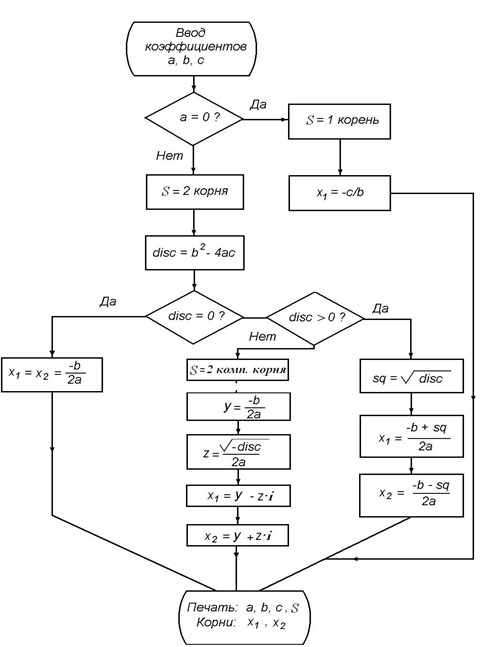
\includegraphics[scale=0.9]{ris_1.jpg}}
\caption{Блок- схема решения квадратного уравнения}
\label{ris1}
\end{figure}

№ 31. {\bf Задача о заряженной капле.}
Капля, обладающая зарядом $Q$, падает на поверхность и раз­деляется на две малые капли $q_1$ и $q_2$, которые, находясь на расстоянии $R$ друг от друга, взаимодействуют с силой $F$. Определить заряд каж­дой из этих капель.

{\it Решение.} Можно заметить, что условию задачи удовлетворяет система уравнений

\begin{equation}
 \begin{cases}
 \begin{aligned}
   q_1 + q_2 = Q\\
   F = \frac{1}{4\cdot\pi\cdot\varepsilon_0}\cdot\frac{q_1\cdot q_2}{R^2}
   \end{aligned}
 \end{cases}
\end{equation}

где ($q_1$ и $q_2$ -- заряды образовавшихся новых капель, 
а диэлектрическая постоянная
 $\varepsilon_0=8.85418782\cdot 10^{-12}$ $\text{Кл}/(\text{В}\cdot m).$
%$A^2\cdot c^4/(m^3\cdot kg)$

Преобразуем систему (1) к виду  

\begin{equation}
 \begin{cases}
 \begin{aligned}
   q_1 + q_2 = Q\\
   q_1\cdot q_2 = {4\cdot\pi\cdot\varepsilon_0}\cdot F\cdot R^2
      \end{aligned}
 \end{cases}
\end{equation}

Полученные уравнения соответствуют требованиям теоремы Виета к корням $x_1$ и $x_2$ квадратного уравнения 
$a\cdot x^2 + b\cdot x +c = 0:$
\begin{equation}
 \begin{cases}
  \begin{aligned}
   x_1 + x_2 = -b/a\\
   x_1\cdot x_2 = c/a, 
      \end{aligned}
 \end{cases}
\end{equation}

т.е. система уравнений (2) эквивалентна квадратному уравнению
$$x^2 - Q\cdot x + 4\cdot\pi\cdot\varepsilon_0\cdot F\cdot R^2 = 0,  \hspace{200pt} (4)$$
    корнями которого будут заряды $q_1$ и $q_2$.
 
Напишите программу, реализующую этот алгоритм, и, по приведенным данным, найдите заряды капель. Для решения уравнения (4) следует использовать программу решения квадратного уравнения, написанную для задачи № 30.

№ 32. {\bf Мячик на плоскости.}
Теннисный мяч подбросили вертикально вверх со скоростью $V_n$. Он поднимется до высоты $H$, после чего начнет падать вниз.\\
При ударе об пол он потеряет $K$ --ую часть энергии, после чего вновь подниматься вверх. Так будет до тех пор, пока мяч не остановится.\\
{\em Задание:} Рассчитать движение мяча и построить картину его движения! Показать на графиках, как изменяется со временем высота подъема мяча, его скорость и кинетическая энергия. Изобразить на левой части экрана динамическую картинку подпрыгивающего мяча, а справа зависимости  $H= H(t)$, $V= V(t)$ и фазовую траекторию $V= V(H)$.

№ 33. {\bf Движение тел, брошенных под углом к горизонту} Рассчитать и нарисовать движение 3-х тел, брошенных под углами $\alpha_1 =30^\circ, \alpha_2 = 45^\circ, \alpha_3 =60^\circ$.  Рассчитать движение $п$ тел, брошенных с одинаковой скоростью   $V_0=50$ м/с  и с близкими углами: $\alpha_1 = 50^\circ, \alpha_2 = 51^\circ, \alpha_3 = 53^\circ$.

№ 34. {\bf Баскетбол.}
Спортсмен ростом $h$ бросает баскетбольный мяч в корзину, установленную на высоте $H$ и находящуюся от него на расстоянии $L$. Начальная скорость броска равна $V_0$. Рассчитайте и нарисуйте возможные траектории мяча. На экран выведите рассчитанные значения углов бросания.\\
Для этого составьте уравнение движения мяча. (Оно -- квадратное относительно $tg(\alpha)$.)  Решите его, используя подпрограмму решения квадратного уравнения.

Траектории мяча должны изображаться на всей плоскости экрана, при любых входных данных. Входными данными задачи  вляются  $V_0$ и $L$.

№ 35. {\bf Шарик на наклонной плоскости.}
Шарик массой m скатывается по наклонному жёлобу, заканчивающемуся "мёртвой петлёй" радиуса $R$ (см. рисунок \ref{ris2}). 
\begin{figure}[!hb]
\centerline{
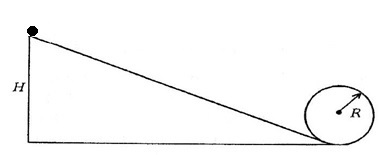
\includegraphics[scale=1.0]{ris_2.jpg}}
\caption{Рисунок к задаче №35}
\label{ris2}
\end{figure}
Шарик начинает движенте по жёлобу без начальной скорости с высоты $H$. Размер шарика $r \ll R$. Построить траекторию движения шарика при различных значениях $H$ и $R$. вводимых по запросу программы.

\subsection{Операции с символами}

Написать программы, которые

№ 36. Вводит строку и разбивает её на слова.

№ 37. Вводит произвольный текст, затем заменяет в нем букву "о" на   символ "*" и получившийся текст выводит на экран.

№ 38. Вводит произвольный символ и выводит его на экран внутри ромба с вершинами на серединах сторон экрана.

№ 39. Вводит произвольный символ и выводит его на экран вне ромба с вершинами на серединах сторон экрана.

№ 40. Форматирует абзац текста любой длины, набранный моноширинным (все буквы имеют одну и ту же заданную ширину), шрифтом.

\subsection{Графика}

№ 41. Изобразить траектории некоторых точек колеса радиуса $R$, катящегося без проскальзывания по рельсу, находящемуся на высоте $H$. Рассмотреть случаи, когда расстояние точки от оси колеса $\rho = 0.5\cdot R, \rho = R, \rho = 1.5\cdot R$. Одновременно с траекториями нарисовать движение колеса.

№ 42. Нарисовать траекторию точки $M$, лежащей на стержне длины $L$ на расстоянии $(L- A)$ от его верхнего конца. Стержень скользит без трения по сторонам прямого угла, причем координата нижнего конца стержня изменяется по закону $x = x_0\cdot\cos(\omega\cdot t)$.

№ 43. Написать программу построения графика произвольно заданной функции. График изображается (в экранных координатах) в прямоугольной системе координат и располагается на экране при любых значениях переменных решаемой задачи (метры, километры, мили, тонны, фунты стерлингов, доллары и т.д.). Оси координат оцифрованы и подписаны. Название функции отображается над графиком.

Программа построения графика должна быть оформлена в виде модуля-подпрограммы так, чтобы её можно было использовать в других программах.

№ 44. Построить график функции
$$y(x)= 1/(3\cdot x^2-1), x \in[-2,2.5]$$

№ 45. На одном экране в двух разных окнах построить два графика сложения гармонических функций, зависящих от параметра $t$. В первом выводится результат сложения колебаний, происходящих в двух взаимно перпендикулярных направлениях --- (фигура Лиссажу),
$$F_1(t) = \sin(k_1\cdot t), \:F_2(t) = \cos(k_2\cdot t).$$
Во втором окне изображается результат сложения двух колебаний, происходящих в одной плоскости (биения)
$$F_3(t) = \sin(k_3\cdot t) + \cos(k_4\cdot t), \:F_4(t) = t$$
$$t\in [-n\cdot \pi, n\cdot \pi], \:n = 1,2,\cdots, 10.  $$

№46. Построить кривые, зависящие от параметра $t:$\\

 1) Улитка Паскаля.\\
$$x = a\cdot \cos^2(t) + b\cdot \cos(t);$$
$$ y = a\cdot \cos(t)\cdot\sin(t) + b\cdot\sin(t).$$
$$a > 0, \:b > 0,\: t \in[0,\:2\cdot \pi]$$

Рассмотреть случаи, когда $b > 2\cdot a, \: a < b < 2\cdot a, \: a > b.$

2) Эпициклоида.\\
$$x = (a + b)\cdot\cos(t) - a\cdot\cos((a + b)\cdot t / a),$$
$$y = (a + b)\cdot\sin(t) - \cdot\sin((a + b)\cdot t / a), $$
$$a > 0,\: b > 0.$$
Рассмотреть случаи, когда $b / a = 3$ и $b / a = 3 / 2.$

3) Строфоида.\\
$$x = a\cdot(t^2 -1)/(t^2 + 1), \:y = a\cdot t(t^2-1) / (t^2 +1).$$
$$ t \in (-\infty ,\:\infty),  a > 0.$$

Построение каждой из кривых должно быть описана как отдельная процедура или функция.


№ 47. Написать программу, рисующую шахматную доску. На доске разместить шашки, причём цвет шашек в верхней части доски отличен от цвета шашек в нижней части.

Шашки размещать на доске с помощью процедур, работающих с памятью. Сначала рисуется шашка, затем её изображение записывается в память ПК, потом извлекается из памяти и устанав­ливается в нужное место.

№ 48. В графическом режиме промоделировать жизнь поко­лений гипотетической колонии живых клеток, которые выживают, размножаются или погибают в соответствии со следующими прави­лами.

Клетка выживает, если и только если она имеет двух или трёх Соседей из восьми возможных (см. рис. а).
 
Если у клетки только один сосед или вовсе ни одного, она поги­бает от "одиночества" (см. рис. б)

Если клетка имеет четырёх или более соседей, она погибает от "перенаселения" (см. рис. в).

В любой пустой позиции, у которой ровно три соседа, в следу­ющем поколении рождается новая клетка (см. рис. \ref{ris3}).
\begin{figure}[!hb]
\centerline{
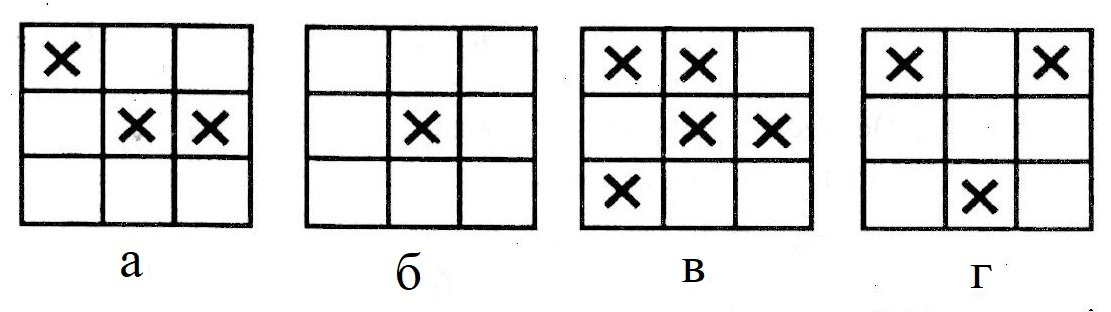
\includegraphics[scale=0.4]{ris_4.jpg}}
\caption{Рисунок к задаче № 48}
\label{ris3}
\end{figure}

{\it Замечание:} Исходная позиция порождается либо в режиме вво­да данных с клавиатуры, либо с помощью датчика случайных чисел, а вместо крестиков можно просто закрашивать клеточки.

№ 49. Написать программу, отображающую на экране монитора циферблат часов со стрелками (ROLEX) и движение стрелок, включая секундную. Программу написать без заметного для глаза мерцания экрана при движении секундной стрелки.

\subsection{Разные задачи}

1. Написать программу, рассчитывающую календарь для любого заданного года (с учетом високосного года), и отобразить его на экране по месяцам.

2. Задача Леонардо на числа Фибоначчи. "Некто поместил пару кроликов в некоем месте, огороженном со всех сторон стеной, чтобы узнать, сколько пар кроликов родится при этом в течение года, если природа кроликов такова, что через месяц пара кроликов производит на свет другую пару, а рождают кролики со второго месяца после своего рождения". Вывести на экран начало получив­шегося числового ряда.

3. На краю поля лежат 100 арбузов. Вы хотите выбрать арбуз с самым большим весом. Как бы Вы осуществили свое намерение? Разумеется, в Вашем распоряжении имеются весы. Возможен и другой путь.
    
4.Некий цех выпускает металлические стержни. Для проверки их качества взяли 50 экземпляров. Стержень считается стандартным, если е$B$. В противном случае изделие считается браком. Требуется подсчитать количест­во стандартных стержней и массу всех бракованных изделий.

Формула для расчета массы:   $$m = \frac{\pi\cdot d^2\cdot l\cdot \rho}{4}, $$
где $d$ -- диаметр, $\rho$ -- плотность,   $l$ -- длина стержня.

5. Реализовать в виде программы алгоритм Евклида.

6. Чтобы обеспечить население города картофелем, его следу­ет закупить в количестве 3000 т в четырех агрофирмах. Количест­во картофеля, которое может продать каждая агрофирма, и цена одной тонны приведены в таблице.

\begin{center}
\begin{tabular}{ | l | l | l |  l |  l |} \hline
Агрофирма & I  &  II  &  III  &  IV   \\   \hline
Объем продаж & 1100  &  900  &  800  &  700   \\   \hline
Цена перевозки &    &     &     &      \\   
одной тонны & 3  &  2.5  &  2  &  2.7     \\   \hline
\end{tabular}
\end{center}
\vspace{5mm}

Разработайте план закупки картофеля и найдите затраты на его перевозку.

7. Напишите программу, вычисляющую полином вида:

$$ p = \frac{x^0}{0!}+\frac{x}{1!}+\frac{x^2}{2!}+ \ldots + \frac{x^n}{n!} = 1 + x + \frac{x^2}{2!} + \ldots + \frac{x^n}{n!}  \approx e^x$$


для различных значений $n$ (меньше и больше 100). Сравните полученный результат с результатом вычисления функции exp(x).


8. Напечатать в порядке возрастания все простые несократимые дроби, заключенные между 0 и 1, знаменатели которых не превышают 7.
    
9. Написать программу, рисующую окружность заданного радиуса и с заданными координатами центра, не пользуясь стандартными средствами PASCAL. Сравнить полученный результат с использованием стандартной процедуры (построения сделать на одном экране).

Написать и запустить на счет программу, которая бы:

11. Отвечала, делится ли введенное число $a$ на введенное число $b$.

12. Отвечала, можно ли введенное натуральное число предста­вить в виде суммы двух квадратов.

13. Определяла, является ли введенное число простым.

14. Вычисляла $n$ -- ый член ряда Фибоначчи, используя рекур­рентную последовательность вида: 
$a_0 = 1, a_1 = 1, \ldots ,a_{n+2} = a_n + a_{n+1}.$

    15. Отвечала, какое максимальное число бутылок лимонада можно выпить, имея $n$ рублей (сумма запрашивается программой).
    
{\it Предполагается, например, что бутылка лимонада стоит 12 рублей, пустая бутылка сдается за 3 рубля и полученные деньги вновь пускаются на приобретение лимонада.}

16.	Рисовала в графическом режиме прямоугольник и изображала движение в нем шарика, зеркально отражающегося от границ этого прямоугольника.

17. Нарисовать траекторию точки $M$, лежащей на стержне длины $L$ (см. рис. \ref{ris4}). Стержень скользит по сторонам прямого угла. \\
{\it Дополнение:} Пусть координата точки $B$  меняется по закону 
$x = x_0\cdot\cos(\omega\cdot t).$
   
\begin{figure}[!hb]
\centerline{
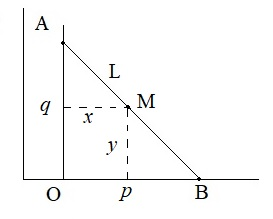
\includegraphics[scale=0.9]{ris_3.jpg}}
\caption{Рисунок к задаче № 17}
\label{ris4}
\end{figure}
 

\section{Заключение}

 %\end{document}

 %\begin{center}
 %     \includegraphics[width=100mm]{comp.jpg}
 %\end{center}
%\newpage
% \begin{figure}[!hb]
% \centerline{
% 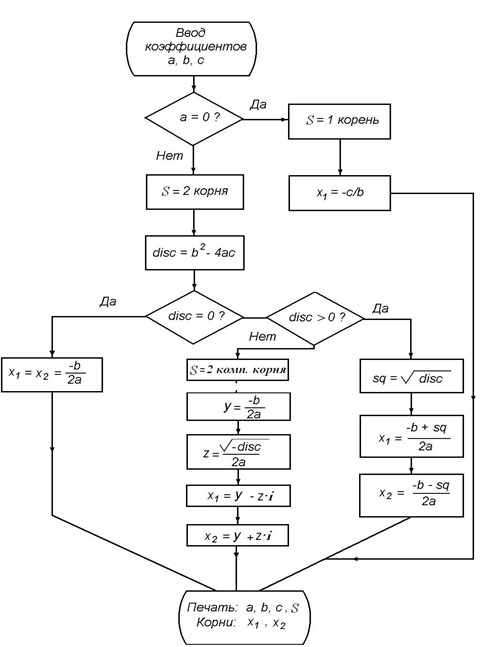
\includegraphics[scale=1.1]{ris_1.jpg}}
% \caption{Рисунок к задаче №35}
% \end{figure}

    \thispagestyle{empty}

\begin{center}

Учебное издание

\vspace*{23mm}

{\bf Деменков} Павел Сергеевич,

\vspace{5mm}

{\bf Молородов} Юрий Иванович

\vspace{25mm}


{\large \bf ИНФОРМАТИКА и ИКТ}\\
{\large Введение в современную информатику: \\Задачи}

\vspace*{0.5cm}

Учебное пособие\\

\vspace*{40mm}

Редактор {\it Т.~В.~Иванова}

\vspace {1cm}

{\small
Подписано в печать {20.06.2021 г.}

Формат 60 x 84 \ 1/16. Уч.-изд.~л.~7,5. Усл.~печ.~л.~7.

\vspace{5mm}
Тираж 120~экз. Заказ № \hspace*{8mm}
\vspace{5mm}

Редакционно-издательский центр НГУ.

630090, Новосибирск-90, ул.~Пирогова, 2.}

\end{center}

   
\thispagestyle{empty}

\begin{center}
МИНИСТЕРСТВО ОБРАЗОВАНИЯ И НАУКИ РФ\\[2mm]
НОВОСИБИРСКИЙ   ГОСУДАРСТВЕННЫЙ УНИВЕРСИТЕТ\\[2mm]
 СПЕЦИАЛИЗИРОВАННЫЙ УЧЕБНО-НЕУЧНЫЙ ЦЕНТР
%НОВОСИБИРСКИЙ НАЦИОНАЛЬНЫЙ ИССЛЕДОВАТЕЛЬСКИЙ\\[2mm]  ГОСУДАРСТВЕННЫЙ УНИВЕРСИТЕТ
\end{center}

%\begin{center}
%{\large Специализированный учебно-неучный центр НГУ}
%\end{center}
\vspace{0.46cm}
\begin{center}
{\Large Кафедра дискретной математики и информатики}
\end{center}

\vspace{3cm}
\begin{center}
{\LARGE  П.~С.~Деменков, Ю.~И.~Молородов}
\end{center}

\vspace{1cm}

\begin{center}
{\Large \bf ИНФОРМАТИКА и ИКТ}\\
{\large Введение в современную информатику: Задачи}
\end{center}

\vspace {1mm}


\begin{center}
Учебное пособие\\

\vspace*{42mm}

Новосибирск\\2021
\end{center}

\newpage

\thispagestyle{empty}

\noindent
УДК 681.3.016 \\
ББК 32.973\\
М 75
% \vspace{5mm}

\begin{center}
Рецензент:\\  д-р тех. наук {\it В.~Б.~Барахнин}\\
\end{center}

\noindent


\vspace{2mm}

\noindent
\begin{tabular}{ll}

& \hspace{-3mm}\bf Молородов,~Ю.~И. \\

\hspace{-3mm}\bf В\;752  & \hspace{-3mm}Информатика и ИКТ: {задачи}~: учеб. пособие / П.~С.~Деменков, \\

&\hspace{-3mm}Ю.~И.~Молородов ; Новосиб.~гос.~ун-т.~---~Новосибирск :  \\

& \hspace{-3mm}РИЦ НГУ, 2021.~---~152~с.
\end{tabular}



\vspace{5mm}
\noindent  ISBN \ 978-5-4437-1000-6 \vspace{8mm}
%\vspace{2mm}

В пособие включены формулировки задач, решение которых позволит углубить знания об особенностях программирования на ЯВУ и понять основные принципы построения алгоритмов решения задач.

Пособие будет полезно школьникам физико--математической школы при Новосибирском государственным университетом, изучающим современные программные средства для работы с текстовой информацией:  подготовкой отчетов, рефератов, статей и пр. самостоятельно или под руководством преподавателей, а также преподавателям, проводящим семинарские и практические занятия.


\vspace{3mm}

\noindent   \hfill~{\bf УДК 681.3.016}

\noindent   \hfill~{\bf ББК 32.973}

\noindent   \hfill~{\bf M 75}

\noindent   \center {\it  Издано при финансовой поддержке Минобрнауки РФ\\ грант № 075-15-2019-1459}

\vspace{3mm}

\noindent \hspace*{-15pt} \hfill~\copyright~Новосибирский государственный университет, 2021

\noindent\hspace*{45pt}\copyright~СУНЦ НГУ, 2021

\noindent \hspace{130pt} ~\copyright~П.~С.~Деменков, ~Ю.~И.~Молородов  \\



\hspace*{-350pt}{ISBN}  978-5-4437-1000-6
%\hspace*{62pt}  2021




%\vspace{5mm}

\end{document}
